\documentclass[12pt,a4paper,oneside]{article}

\usepackage[pdftex,
            pdfauthor={Albert Zak},
            pdftitle={Dynamic Software Updating in Erlang/OTP},
            pdfsubject={Bachelor Thesis},
            hidelinks,
            driverfallback=hypertex]{hyperref}
\usepackage[english]{babel}
\usepackage{lmodern}
\usepackage[utf8]{inputenc}
\usepackage[T1]{fontenc}
% \usepackage{arialu}
% \renewcommand{\familydefault}{\sfdefault}
% \normalfont
\renewcommand{\rmdefault}{phv} % Arial
\renewcommand{\sfdefault}{phv} % Arial

\usepackage{microtype}
\usepackage{geometry}
\usepackage{bookmark}
\usepackage{listings}
\usepackage[inline]{enumitem}
\usepackage{subcaption}
\usepackage{tabularx}
\usepackage{multirow}
\usepackage{floatrow, makecell}
\usepackage{hhline}
\usepackage{boldline}
\usepackage{algpseudocode}
\usepackage{stackengine}
\usepackage{tikz}
\usetikzlibrary{trees,arrows,fit,positioning,shapes.geometric,shadows}
\PassOptionsToPackage{usenames,dvipsnames,svgnames,table}{xcolor}
\usepackage{xcolor-solarized}
\usepackage{gitdags}
\usepackage[singlespacing]{setspace}
\usepackage[acronym,nopostdot,style=super,nonumberlist,nogroupskip]{glossaries}
\usepackage{fancyhdr}
\usepackage{hyphenat}
\hyphenation{name-space}
\usepackage{forest}
\forestset{
  dir tree/.style={
    for tree={
      parent anchor=south west,
      child anchor=west,
      anchor=mid west,
      inner ysep=-3pt,
      grow'=0,
      align=left,
      edge path={
        \noexpand\path [draw, very thin, lightgray, \forestoption{edge}] (!u.parent anchor) ++(1em,0) |- (.child anchor)\forestoption{edge label};
      },
      font=\ttfamily,
      if n children=0{}{
        delay={
          prepend={[,phantom, calign with current]}
        }
      },
      fit=band,
      before computing xy={
        l=2em
      }
    },
  }
}

\pagestyle{fancy}
\fancyhf{}
\cfoot{\thepage}
\renewcommand{\headrulewidth}{0pt}

\makeglossaries{}
\newacronym{bif}{BIF}{Built-in Function}
\newacronym{erts}{ERTS}{Erlang Run-Time System}
\newacronym{vm}{VM}{Virtual Machine}
\newacronym{otp}{OTP}{Open Telecom Platform}
\newacronym{sasl}{SASL}{System Architecture Support Libraries}
\newacronym{os}{OS}{Operating System}
\newacronym{vcs}{VCS}{Version Control System}
\newacronym{api}{API}{Application Programming Interface}
\newacronym{ci}{CI}{Continuous Integration}
\newacronym{cli}{CLI}{Command Line Interface}
\newacronym{ram}{RAM}{Random Access Memory}
\newacronym{dsu}{DSU}{Dynamic Software Updating}
\newacronym{tls}{TLS}{Transport Layer Security}
\newacronym{http}{HTTP}{Hypertext Transfer Protocol}
\newacronym{lxc}{LXC}{Linux Containers}
\newacronym{beam}{BEAM}{Bogdan/Björn's Erlang Abstract Machine}
\newacronym{ecs}{ECS}{Elastic Compute Cloud Container Service}
\newacronym{cow}{CoW}{Copy-on-Write}
\newacronym{appup}{appup}{Application Upgrade Instructions}
\newacronym{relup}{relup}{Release Upgrade Instructions}
\newacronym{tmpfs}{tmpfs}{Temporary File System}
\newacronym{nif}{NIF}{Native Implemented Functions}
\newacronym{rest}{REST}{Representational State Transfer}
\newacronym{etf}{ETF}{Erlang External Term Format}
\newacronym{ssh}{SSH}{Secure Shell}
\newacronym{mfa}{MFA}{Module, Function, Arity}
\newacronym{sse}{SSE}{Server-Sent Events}
\newacronym{ip}{IP}{Internet Protocol}


\lstset{
  language=bash,
  numbers=left,
  numberstyle=\small\color{lightgray},
  basicstyle=\ttfamily,
  frame=tb,
  firstnumber=0,
  stepnumber=5
}
% Hide number in first line of code listings
\makeatletter
\def\lst@PlaceNumber{\ifnum\value{lstnumber}=0\else
  \rlap{\normalfont\kern\linewidth \kern\lst@numbersep\lst@numberstyle{\thelstnumber}}\fi}
\makeatother

\pdfpageheight=297mm
\pdfpagewidth=210mm
\geometry{a4paper, left=30mm, right=25mm, top=30mm, bottom=30mm}

\begin{document}

\frenchspacing

\pagestyle{empty}
\thispagestyle{empty}
\begin{picture}(50,50)
  \put(-70,40){\hbox{\includegraphics[width=5cm]{fhcw-logo.pdf}}}
\end{picture}

\vspace*{-5.8cm}

\begin{center}
  \vspace{6.5cm}
  \hspace*{-1.0cm} {\LARGE \textbf{Deployment of Erlang/OTP Releases\\}}
  \hspace*{-1.0cm} {\LARGE \textbf{ \\}}
  \vspace{0.5cm}
  \hspace*{-1.0cm} Implementation of a Node Agent, and Analysis of Failure Modes \\

  \vspace{2cm}

  \hspace*{-1.0cm} {\LARGE \textbf{Bachelor Thesis\\}}
  \vspace{0.65cm}

  \hspace*{-1.0cm} Submitted in partial fulfillment of the requirements for the degree of \\

  \vspace{0.65cm}

  \hspace*{-1.0cm} \textbf{Bachelor of Science in Engineering} \\
  \vspace{0.65cm}
  \hspace*{-1.0cm} to the University of Applied Sciences FH Campus Wien \\
  \vspace{0.4cm}
  \hspace*{-1.0cm} Bachelor Degree Program\\
  \hspace*{-1.0cm} Information Technology and Telecommunications\\

  \vspace{2cm}

  \hspace*{-1.0cm} \textbf{Author:} \\
  \vspace{0.2cm}
  \hspace*{-1.0cm} Albert Zak \\
  \vspace{0.7cm}

  \hspace*{-1.0cm} \textbf{Student identification number:}  \\
  \vspace{0.2cm}
  \hspace*{-1.0cm} 1510475069 \\
  \vspace{0.7cm}

  \hspace*{-1.0cm} \textbf{Supervisor:} \\
  \vspace{0.2cm}
  \hspace*{-1.0cm} Priv.-Doz. Mag.rer.soc.oec.\\
  \hspace*{-1.0cm} Dipl.-Ing. Dipl.-Ing. Dr.techn.\\
  \hspace*{-1.0cm} Karl Michael Göschka \\
  \vspace{0.7cm}

  \hspace*{-1.0cm} \textbf{Date:} \\
  \vspace{0.2cm}
  \hspace*{-1.0cm} 01.06.2018 \\

\end{center}

\newpage

\vspace*{16cm}
\begin{flushleft}
  \underline{Declaration of authorship:}\\
  \vspace{0.5cm}
  I declare that this Bachelor Thesis has been written by myself. I have not used any other than the listed sources, nor have I received any unauthorized help.\\
  \vspace{0.5cm}
  I hereby certify that I have not submitted this Bachelor Thesis in any form (to a reviewer for assessment) either in Austria or abroad.\\
  \vspace{0.5cm}
  Furthermore, I assure that the (printed and electronic) copies I have submitted are identical.\\
  \vspace{1cm}
  Date: \hspace{5.3cm} Signature:
\end{flushleft}


\newpage
\pagestyle{fancy}
\pagenumbering{roman}
\cleardoublepage{}

\section*{Abstract}

Highly available Erlang/\acrshort{otp} systems taking advantage of \acrfull{dsu} require a manual deployment process that is at odds with the practice of \acrlong{cd}. Previous work on automating Erlang/OTP release handling produced tools with imperative semantics that relied on pushing commands via remote shells.

This thesis presents a declarative deployment pipeline capable of \acrshort{dsu} that requires minimal configuration to bootstrap a node. An agent running on a separate emulator subscribes to a central release store, pulls artifacts, and installs them without user interaction. The initial deployment primitive is a generic container into which the node agent pulls new releases during runtime. By treating containers as mutable, the proposed solution combines the \acrshort{dsu} facilities of Erlang/OTP with the ease of deploying containers using existing orchestration tools.

An evaluation of \acrshort{dsu} failure scenarios reveals various sources of possible issues, some of which may be caught through static analysis, and some requiring more research before \acrshort{dsu} can safely be used for general purpose Erlang/OTP systems.


\renewcommand{\glsnamefont}[1]{\textbf{#1}}
\doublespacing
\printglossary[title=List of Abbreviations,nonumberlist,type=\acronymtype]
\singlespacing

\cleardoublepage

\section*{Key Terms}
Continuous Delivery\\
Git \\
Tooling \\
Erlang \\
Elixir \\
Automation \\
Dynamic Software Updating \\

\cleardoublepage

\tableofcontents{}

\cleardoublepage

\pagenumbering{arabic}

\section{Introduction}

The contributions of this work are \begin{enumerate*}[label=(\roman*)]
  \item an extension to the pipeline described in~\cite{zak18} to bootstrap an Erlang/\acrshort{otp} (\emph{\acrlong{otp}}) node with a single command, which pulls artifacts from a central store and deploys them without interaction; and
  \item an analysis of possible failure modes and root causes that may prevent an upgrade from being applied successfully via \acrfull{dsu}.
\end{enumerate*} This section explains relevant terminology and shows where manual interaction is required to deploy \acrshort{otp} Releases.

\subsection{Erlang/OTP}

Erlang is a programming language for building concurrent, distributed systems with high availability requirements. Initially designed by Ericsson for telephone exchanges, it has been embraced by industries with similar needs: finance, gaming, betting, messaging, middleware, and databases. Development of Erlang took place starting in 1986 at the Ericsson Computer Science Laboratory, and in 1998 Erlang was released as Open Source.~\cite{armstrong2007history}

\acrshort{otp} stands for \acrlong{otp}, and is a combination of library applications, design patterns, conventions, and documentation. Erlang is almost always used in conjunction with \acrshort{otp}, hence the name Erlang/\acrshort{otp}.~\cite{ferd}

The language is often described as functional, although it is not strictly side effect free or referentially transparent. Erlang compiles to bytecode, which is executed by a \acrfull{vm}. The current Erlang \acrshort{vm} – the \emph{\acrshort{beam}}, short for \emph{\acrlong{beam}} – is written in C and supports various machine architectures. Multiple languages that compile to \acrshort{beam} bytecode have been created, most famously \emph{Elixir} and \emph{Lisp Flavored Erlang}. Actor model processes are the language's concurrency primitives: Functions can be spawned to create lightweight \acrshort{beam} processes. They are different from \acrfull{os} processes or threads, being preemptively scheduled by the \acrshort{beam}. Erlang/\acrshort{otp} systems commonly ``run millions of processes simultaneously [with each one taking] less than a kilobyte of space.''~\cite{larson}

\paragraph{\acrshort{otp} Applications.}
Erlang code is constructed out of functions defined within \mbox{\emph{module}} files bearing an \lstinline|*.erl| extension. \emph{\acrshort{otp} Applications} group related modules into reusable units to provide well-defined start and stop semantics, including an \emph{application resource file} (\lstinline|*.app|) containing additional metadata such as a version string and a list of other applications that this application depends on, and which need to be started beforehand. Every application has a dependency on at least \lstinline|kernel| and \lstinline|stdlib|, and both must be specified in the application resource file.~\cite{doc:otp}

\acrshort{otp} also enforces a certain directory structure for applications.~\cite{logan:otp}

\paragraph{\acrshort{otp} Releases.} Whole projects consisting of multiple applications are packaged and deployed as \acrshort{otp} Releases. They are described by a release resource (\lstinline|*.rel|) file, which specifies additional metadata, such as a version string for the entire release, the included version of the \emph{\acrlong{erts}} (\acrshort{erts}), and a list of applications with their respective version strings that comprise the release.

From this release resource file, various tools can be used to create a boot script and assemble the release into a single compressed tarball (\lstinline|*.tar.gz|) package.~\cite{doc:otp} A packaged release contains everything necessary to bootstrap an \emph{embedded target system} on another machine, also called a \emph{node}. Depending on the tool used to generate the release, it may include additional convenience scripts to upgrade or inspect the target system.

\paragraph{\acrlong{dsu}.} A core feature of Erlang is its support for \acrfull{dsu}, also referred to as on-the-fly upgrading, or hot code loading. The \acrshort{beam} keeps up to two versions of a module loaded in memory, and both versions of the code may run side by side.~\cite{cesarini:otp} \acrshort{otp} provides generic \emph{behaviours} that \emph{callback modules} can implement to normalize start, stop and upgrade semantics, among others.~\cite{doc:otp} Erlang systems constructed according to \acrshort{otp} patterns, grouped into \acrshort{otp} Applications, and packaged as \acrshort{otp} Releases enjoy additional support for \acrshort{dsu} via instruction files: \emph{\acrshort{appup}s} (\emph{\acrlong{appup}}) and \emph{\acrshort{relup}s} (\emph{\acrlong{relup}}).

First, there are high-level, often handwritten \acrfull{appup} files, one for each \acrshort{otp} Application. These files are fed into release generation tools where they are translated and combined into a single low-level \acrshort{relup} file, thus making a given release \acrshort{dsu}-capable.~\cite{doc:otp} The \acrshort{relup} file contains instructions on how to upgrade a node running a previous version. A single release package can include one \acrshort{relup} file which may know how to upgrade from multiple previous releases. These files also contain instructions on how to downgrade to the previous version in case the upgrade fails.~\cite{doc:otp}

\subsection{Problem}\label{sec:problem} Most existing release generation tools require manual interaction at various steps, and are generally not trivial to set up and use out of the box in a noninteractive build environment, such as a \acrfull{ci} pipeline. Additionally, there are some pitfalls when developers assemble releases on, for example, their \emph{macOS} development machines and then attempt to start them on \emph{Linux} in production~\cite{cesarini:otp}: This fails with a nonobvious error. To generate an \acrshort{otp} Release capable of \acrshort{dsu}, a developer needs to manually write \acrshort{appup} files and increment version numbers for all changed applications. The \acrshort{otp} Release resource file has an additional, separate version number that needs to be updated between commits to be able to perform \acrshort{dsu}. Then, to generate upgrade instructions, previous releases need to be fetched and unpacked. Lastly, the developer has to invoke various commands to assemble the final release package tarball.~\cite{ferd}

This process is tedious to perform manually, and impedes frequent deployment of small changes. Likewise, complex code changes are more likely to fail when applied via \acrshort{dsu}.~\cite{hicks} The unfortunate consequence is that developers are discouraged from using Erlang's \acrshort{dsu} capabilities unless absolutely necessary.~\cite{ferd}

\subsection{Contribution}

This work contributes design, implementation and evaluation of an extension to the build tool described in~\cite{zak18} for deploying Erlang/\acrshort{otp} Releases with support for \acrshort{dsu}. Its aim is to run without user interaction and to require as little configuration as possible. Additionally, the evaluation includes an analysis of \acrshort{dsu} failure modes.

\paragraph{Goal.} The goal is to develop a prototype implementation for bootstrapping an Erlang node with a single command. The node agent subscribes to the previously described release store to fetch release packages, download, extract, and deploy them; as well as apply \acrshort{dsu} instructions.

\paragraph{Method.} The thesis describes the architectural and design decisions made while iteratively implementing said node agent. The prototype is then used to tests the boundaries of the \acrshort{dsu} process. Finally, the work discusses limitations and advantages of the implementation.

\cleardoublepage
\subsection{State of the Art}\label{sec:sota}

The proposed tool, \emph{BeamUp}, relies on several layers of existing tooling, as visualized in Figure~\ref{fig:tools}. At the lowest level, Erlang/\acrshort{otp} ships with the \acrfull{sasl} that include the two basic building blocks for \acrshort{dsu} support: \lstinline|systools| provides low-level functions for \emph{offline} release generation, and \lstinline|release_handler| is used to perform an \emph{online} hot upgrade of a running node.~\cite{doc:otp}
Elixir projects are built with \lstinline|mix| (not pictured) and releases are generated with \lstinline|distillery|~\cite{distillery}, which handles generation of upgrade instructions itself, and directly interacts with \lstinline|systools|. Erlang projects, however, need more coaxing: Modules and dependencies are compiled with \lstinline|rebar3|, \acrfull{appup} files are generated on a best-effort basis by comparing \acrshort{beam} bytecode via a plugin to \lstinline|rebar3|~\cite{rebar3appup}, while release assembly is done by another intermediary tool, \lstinline|relx|~\cite{loder2016production}.

\vspace{2cm}
\begin{figure}[h]
  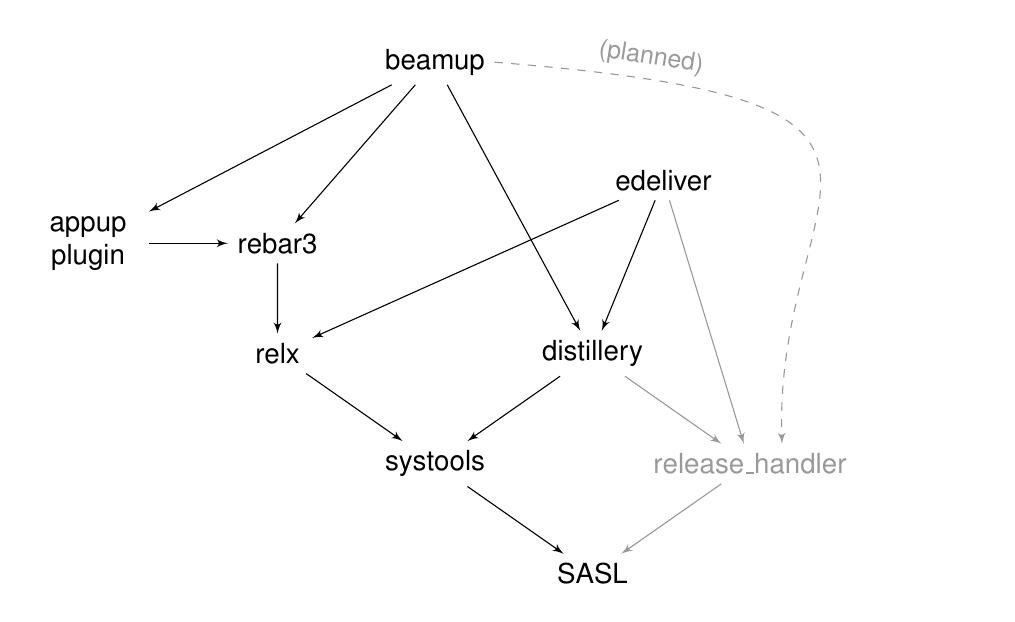
\begin{tikzpicture}[sibling distance=40mm,
    level distance=14mm,edge from parent,>=latex']
    \tikzstyle{edge from parent}=[draw,<-]
    \node (edeliver) at (0.9, 5) {\lstinline|edeliver|};
    \node (beamup) at (-2, 6.5) {\lstinline|beamup|};

    \node {\lstinline|SASL|} [grow'=up] {
      child {node {\lstinline|systools|}
        child {node (relx) {\lstinline|relx|}
          child {node (rebar3) {\lstinline|rebar3|}}}
        child {node (distillery) {\lstinline|distillery|}}}
      child {node (release_handler) [text=black!40] {\lstinline|release_handler|} edge from parent[draw=black!40]}
    };

    \node (appup) [left=10mm of rebar3,text centered,text width=13mm] {\lstinline|appup| \lstinline|plugin|};

    \draw[->] (appup) -- (rebar3);

    \draw[->] (edeliver) -- (distillery);
    \draw[->] (edeliver) -- (relx);
    \draw[->,draw=black!40] (edeliver) -- (release_handler);
    \draw[->,draw=black!40] (distillery) -- (release_handler);

    \draw[->] (beamup) -- (distillery);
    \draw[->] (beamup) -- (rebar3);
    \draw[->] (beamup) -- (appup);
    \draw[->,dashed,draw=black!40] (beamup.east) .. controls (5,6) and (2.3,5) .. node[very near start,sloped,above,text=black!40] {\small{(planned)}} (release_handler.32);

  \end{tikzpicture}
  \caption{Dependencies between selected tools to create and handle releases.}\label{fig:tools}
\end{figure}

\cleardoublepage
\section{Related Work}\label{sec:related_work}

There have been several attempts to automate Erlang/\acrshort{otp} release generation.

\emph{Sinan}~\cite{sinan} was a widely used tool to simplify assembling releases, but did not automate generation of \acrshort{appup}s. The project is deprecated since 2012.

\emph{Knit}~\cite{davis:knit,davis:talk} aimed for simple operation; requiring just one command to generate a \acrshort{dsu}-capable release from previous packages. Knit relied on the build tool \lstinline|rebar|, which–-unlike its successor \lstinline|rebar3|---included an algorithm similar to~\cite{rebar3appup} for generating \acrshort{appup}s. Knit optionally took metadata hints from the developer via \emph{module attributes} to guide \acrshort{appup} generation. The project was last updated in 2014 and appears to be abandoned.

\emph{Relflow}~\cite{relflow} integrates with the Git \acrfull{vcs} and automatically versions releases by rewriting the \lstinline|rebar3| config file. It uses its own \acrshort{appup} generation algorithm that relies on Git to detect what modules have changed between versions.

\emph{Tetrapak}~\cite{tetrapak} is an alternative release assembling tool that outputs artifacts as Debian packages. It too supports configurable automated versioning from \acrshort{vcs} commits, but has no support for \acrshort{dsu}.

\emph{Edeliver}~\cite{edeliver,talk:edeliver} shares very similar goals to the proposed tool. It supports Erlang and Elixir projects, coaxing any of the following tools used on a project: \lstinline|rebar|, \lstinline|relx|, \lstinline|exrm|, or \lstinline|distillery|. It generates releases capable of \acrshort{dsu} with configurable autogenerated version strings. To provide a repeatable build environment, Edeliver opens a \acrfull{ssh} tunnel to a separate build host and assembles the release remotely. Written in \lstinline|bash|, it has no additional dependencies. The tool also handles deployment via \acrshort{ssh}, including remotely performing \acrshort{dsu}.

A different approach to release assembling relies on \emph{Nix}, a general purpose package manager borrowing ideas from functional programming: immutability, pure functions, and referential transparency.~\cite{nix1} Its artifacts are identified via cryptographic hashes of all inputs used to build them. Nix provides repeatable environments to build packages in, similar to what containers are used for in this work, but with stronger determinism. Nix forms the base of \emph{NixOS}~\cite{nixos}, a full featured Linux distribution where almost all components are controlled by Nix via symbolic links.

Previous work by~\cite{erlangnix} allows dependencies of Erlang/\acrshort{otp} projects to be managed via Nix, relying on \cite{hex2nix} to provide Nix metadata, called \emph{Expressions}, for most of the Erlang and Elixir packages hosted on \lstinline|hex.pm|, the primary package repository of the Erlang/\acrshort{otp} ecosystem. Lastly,~\cite{erlangnix2}~presents a pipeline to deploy Erlang/\acrshort{otp} projects using Nix.

\section{Implementation}

The contribution of this work is an extension to the tool \emph{BeamUp}~\cite{zak18} for bootstrapping an Erlang node to start an OTP Release with a single command, and to continuously apply Release Upgrades to the running system without user interaction using Erlang/OTP's built-in support for \acrshort{dsu}. The \emph{node agent} is written in Erlang, and runs on a separate \acrshort{beam} instance side by side to the \emph{operational node}. The agent subscribes to a central store to fetch release packages, caches them locally, and boots, controls, and monitors the operational node.

% TODO: Figure of the two BEAMs

\begin{figure}[h]
  \centering
  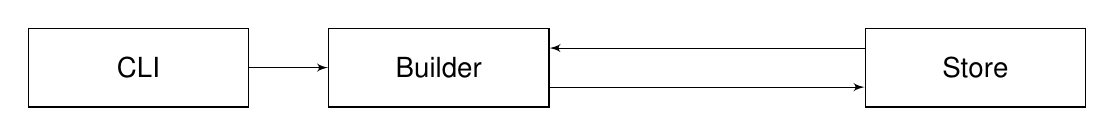
\begin{tikzpicture}[>=latex']
    \tikzset{block/.style={
      draw,
      rectangle,
      align=center,
      minimum width=2.8cm,
      minimum height=1cm
    }};

    \node [block] (cli) {CLI};
    \node [block, right=1cm of cli] (builder) {Builder};
    \node [block, right=4cm of builder] (store) {Store};

    \path[draw,->] (cli) edge (builder);
    \path[draw,<-] (builder.10) -- (store.170);
    \path[draw,->] (builder.350) -- (store.190);

  \end{tikzpicture}
  \caption{Architecture outline.}\label{fig:impl}
\end{figure}

The following subsections explain the changes made to the release store and \acrshort{cli} tool, the bootstrapping process, how the node agent is implemented, and how the agent interacts with the operational node.

\subsection{Store}


\paragraph{Release name.}
OTP has no notion of a project; the most coarse level of organization is a Release, which is given a name. Multiple distinct Releases comprising different Applications may be generated from a single codebase, each bearing a unique name. For example, individual nodes in a distributed setup may run separate Releases with distinct configurations. The build tool described in~\cite{zak18} ignored this fact and generated only one release, always picking the name of the containing folder (the project name) as the name for the release. An artifact was identified by the combination of project name, release version, machine architecture, and git branch. All \acrshort{api}s now additionally take into consideration the release name, defaulting to the project name if left unspecified.

\paragraph{Notifications.} The store now provides an additional endpoint through which nodes can subscribe to be notified when new artifacts are available. The notification system is based on the \acrfull{sse} standard, with the payload message encoded in \acrfull{etf}. Decoding the update notification yields a tagged tuple containing the just latest version string. The new binary release package needs to be fetched separately via the existing single artifact \acrshort{http} GET endpoint.

\ffigbox[\textwidth]{
  \vspace{8pt}

  \lstinline|GET|\hspace{0.3em}\lstinline|/|$\langle$\emph{project name}$\rangle$\lstinline|/|release\lstinline|/|$\langle$\emph{release name}$\rangle$\lstinline|/|$\langle$\emph{architecture}$\rangle$\lstinline|/|$\langle$\emph{branch}$\rangle$

  \vspace{8pt}

  Content Type: \lstinline|application/erlang|

  \acrfull{etf}

  \vspace{8pt}

  \lstinline|\{latest_version, Vsn::binary\(\)\}|

  \vspace{8pt}
}{\caption{Supplementary \acrshort{sse} \acrshort{api} of the store.}\label{fig:api_list}}


\subsection{Bootstrapping}
The invocation of the \acrshort{cli} tool to start a node running the latest version of a particular project is given in Listing~\ref{lst:node}. The node is pointed at the release store via environment variables, optionally supplying a shared authentication token, and is told what project and optionally what release name to run. Note that this command only needs to be run once, except after a reboot of the host. The node subscribes to the store to be notified of new versions, and downloads and applies them without user interaction.

\begin{lstlisting}[
  label={lst:node},
  caption={Minimal node bootstrap command.}
]
BEAMUP_NODE_PROJECT_NAME=mychat \
BEAMUP_STORE=https://store.example.com \
beamup node
\end{lstlisting}

\paragraph{Transparent container invocation.}
All \lstinline|beamup| \acrshort{cli} commands are either executed directly on the host, or, if possible, passed into a newly started container where they run in a well-defined environment. If it is not possible to start containers –– which is the case if the tool is being started inside an already-running container –– then it must assume that the \acrshort{erts} is  set up correctly on the machine. This is why the tool prefers to pass execution into a well-known container, where the same command is then ran again. Once inside, the tool can safely proceed under the assumption that the environment is correct.~\cite{zak18}


\paragraph{Container privileges.}
The container is started in privileged mode and with host networking. This means that no port mapping is required or even possible. The container shares the same \acrshort{ip} address as the host, and can listen on all unprivileged ports except those used by other programs running on the host. The same applies to other devices attached to the host machine, they are accessible from within the container. The advantage of starting the node with this command is its simplicity, as the fact that the operational node is running inside a container becomes mostly transparent to the user.

\paragraph{Bare node container.}
The command in Listing~\ref{lst:node} is not suitable for deploying more complex services, as there is no way of arbitrarily accessing the host's file system, or restricting access to the host's devices. At the same time, the container has access to the host networking stack, which poses a security risk because the container can write to, for example the host's D-bus.~\cite{docker:docs}

For production deployments, it is thus recommended to start the provided general purpose \lstinline|beamup/node| container from the Docker Hub and configure its privileges and port mappings accordingly using any container orchestration tool. Doing so has the additional advantage of locking down the container's environment and communication capabilities in a declarative way.

When the container is started, the same node command is invoked inside. Note that the version of Erlang/OTP which ships with the image is only relevant to the node agent, because the operating node will use the version of the \acrshort{erts} bundled with the release package, and the two \acrshort{beam}s running inside a node share nothing.

\paragraph{Environment variables}
% Table

\paragraph{Node identification}
% Cookie, Node name


\subsection{Release Packages}

The node agent maintains two persistent directories which are mapped to the host file system: \begin{enumerate}[label=(\roman*)]
  \item a local cache of release package tarballs in \lstinline[breaklines=true]|~/.beamup/node/releases|,
  \item and one operating directory containing the current target system in \lstinline[breaklines=true]|~/.beamup/node/active|.
\end{enumerate}

On startup, the agent attempts to start a node from the operating directory. In case of a first run, or when there is no valid release found inside the operating directory, the supervising process yields. If an operational node can be started, the agent does not yet care what version it is running.

In any case, the agent meanwhile connects to the store and retrieves the latest version metadata of the requested combination of project name, release name, machine architecture, and git branch.

When the latest version happens to be the same as the one inside the operating directory, it has already been started and no further action is needed. Otherwise, the latest package is either fetched from the local release cache, or downloaded and stored before it is unpacked to the operating directory.

If there is no latest version of the requested artifact present in the remote store, the agent prints a warning and yields. Nonetheless, it subscribes to be notified when a matching package is published.


\paragraph{Extracting release packages.}
When unpacking a release, the agent must take care to use the correct method: If the operating directory contains a valid target system, the agent must call the release handler of the operational node to properly unpack the new release on top of the currently running one. This is important because the \lstinline|RELEASES| file in the operating directory contains metadata about all of the releases that are currently available to the node. Yet the release package which is to be extracted on top of the operating folder contains another \lstinline|RELEASES| file, which may not overwrite the existing one. Their contents must be properly merged by the release handler, as the new release will be marked as ``unpacked, but not yet installed'', and the old release metadata must remain inside this file. The release handler also performs some sanity checks for missing files on the release package before extracting. On the other hand, if there is no target system available in the operating folder, the package is simply unpacked using \lstinline|tar|.

\subsection{Node Agent}

The node agent is responsible for starting and upgrading the operational node. It runs on a separate instance of the \acrshort{beam} side by side to the operational node, and is designed to be minimally intrusive. Communication only happens via the target system's exposed convenience scripts inside its \lstinline|bin| directory. When a release is to be upgraded, for example, the node agent spawns another OS-level process of the system's shell, calling the \lstinline|bin/upgrade| script with the required parameters, and waiting for it to terminate. This
degree of separation may appear inefficient, as the node agent could just join the operational node using a hidden shell and directly interact with the release handler. Yet, by only assuming the existence of the informal \acrshort{api} exposed by the scripts in \lstinline|bin|, whatever tool used to assemble the release can define exactly how the upgrade should take place.



The node agent does not listen on any ports, and does not attempt to join other agents or the operational node's cluster by default. This is to allow the operational node to transparently interact with the host's networking stack by not causing unexpected port collisions when the node is started via the convenience command.


\paragraph{Attaching a shell.}
To perform tracing on a live system, administrators can attach a shell to either the node agent or


\subsection{Release Upgrades}

\subsection{Synchronized Rollback}
When hot upgrading a distributed system, it is often desirable to minimize the time where different versions of the code are in concurrent use.

\cleardoublepage
\section{Discussion}

The following two sections qualitatively review the contribution with respect to the stated goals, and expose limitations of the current implementation as well as discuss flaws inherent to the design.

\subsection{Advantages}

\paragraph{One time setup.} The tool is meant to be used as part of a \acrfull{ci} pipeline. Invoking a single command generates a deployable artifact from a checkout of the code base. Version identifiers are constructed out of commit timestamps and hashes, and \acrfull{appup} are generated on a best-effort basis. Previous releases are fetched from a central store, where the newly generated release artifact is uploaded to.

\paragraph{.} The \acrshort{cli} build tool is installed with a single command that does not need super user permissions, is not dependent on any specific package manager, and has no dependencies except \lstinline|curl|, \lstinline|bash| and Git––which can safely be assumed to exist on the system.

\paragraph{\acrshort{ci} support.} The tool has been shown to work on at least six common hosted \acrfull{ci} providers: \emph{Travis \acrshort{ci}, Codeship, Circle \acrshort{ci}, Wercker, Semaphore,} and \emph{Shippable}. Build run time and setup effort are comparable across providers.

\paragraph{Declarative.} The command to start a build is always the same, there are no flags or parameters. All settings such as authentification credentials for the store, or the version of Erlang/Elixir to use are passed to the tool via environment variables. The build process requires no interaction.

\paragraph{Single cache.}  Instead of having to configure and maintain multiple cache paths that may change in the future, the cache locations of various tools used within the build process are consolidated inside one directory.

\paragraph{Normalized environment.} The tool detects whether it is being run directly on a \acrshort{vm}, in which case it attempts to normalize the environment by starting a container. Nevertheless, the tool aims to be well behaved with respect to its environment.

\paragraph{Read only.} The tool never modifies the original project folder. All operations happen on temporary copies, preferably on a \acrshort{ram} disk, and the only artifact produced by a build run is a single deployable tarball. The compressed release artifact is either directly uploaded to a remote store, or written to the file system as specified by an environment variable.

% --
\cleardoublepage
\subsection{Limitations}

\paragraph{Installer.}\label{sec:curlpipesh} Distributing the \acrshort{cli} tool by downloading a script and piping it to the shell, thereby immediately executing its arbitrary contents may appear to be unsafe. Yet there is currently no simpler solution. The content delivery network that serves the installer script is configured to only accept connections over \acrshort{http}S, and \lstinline|curl| verifies the validity of the certificate. The installer is wrapped in a shell function to guard against executing a partially downloaded script. Besides, those concerned about the security implications can circumvent the installer by manually cloning a vetted checkout of the \acrshort{cli} repository.

\paragraph{Linux only.} Since the build process always runs inside a Linux container, the resulting release artifact only runs on Linux systems as well. Note that the \acrshort{cli} tool itself may be invoked on other \acrshort{os}s where Docker is supported, such as macOS, as the Docker client will then transparently run the container on a virtualized Linux kernel.~\cite{docker:docs} Consequently, the built release still only supports Linux.

\paragraph{Minimal customization.} The tool aims to cover only the most common default project configurations. This implies that all configuration files for the respective tools are in their standard locations, and that the project is set up like the scaffolding generated by the \lstinline|beamup new| command. Advanced features of the build tools such as build profiles, native dependencies, or multiple releases are not supported.

\paragraph{Already containerized pipeline.} All but one of the tested \acrshort{ci} providers run the build inside a preconfigured container, with only Travis \acrshort{ci} offering the choice between a container or a \acrshort{vm}. When the container has already been started, the launcher cannot make certain optimizations. Namely, it cannot mount a \acrshort{tmpfs} \acrshort{ram} disk, or consolidate the cache folders. The tool must also assume that the correct version of Erlang/\acrshort{otp} is already installed.

\paragraph{High \acrshort{ram} or disk usage during build.}
To avoid disk thrashing and to improve performance, the tool attempts to copy the project folder onto a \acrshort{ram} scratch disk. This working copy is naively duplicated multiple times during the build process, at least twice for every upgrade from a previous release. Note that in case the \acrshort{ram} disk fills the available memory, the \acrshort{os} falls back to using swap space. Nevertheless, the builder attempts to keep the number of concurrently existing duplicates to a minimum.


\paragraph{Store is an active component.} The builder currently supports two backends for storing built artifacts. The release tarball may either be output to the local file system, or uploaded to the store, which is an active server component that must be deployed and maintained. The current feature set implies that an active store component is unnecessary, and a backend for e.g.~a simple object storage would suffice.

The \acrshort{api} and implementation of the store server is incomplete and will in the future be extended to cover additional aspects of release handling, deployment and bootstrapping of nodes.

\paragraph{Possibly unnecessary downloading of previous releases.} The tool currently downloads the entirety of all previous releases to generate upgrade instructions. An alternative would be to locally check out the previous commits to upgrade from, compile each previous release from the checked out code, and then to compare them to generate upgrade instructions, as documented by~\cite{rebar3appup}. This paper has not evaluated advantages or limitations of a local-only approach.

\paragraph{Releases contain debug information.} Expanding the point made above, the current approach might be flawed in the following way: To generate upgrade instructions from previous releases, the bytecode files needed to be compiled with included debug information. This can be used to reconstruct the Erlang source code.~\cite{doc:otp}

\paragraph{Transient network failures.} Out of 448 test runs, three failed. Two failed attempts to download a dependency could have been caught and retried by the build tool. Retrying on network failures should arguably be a concern of the lower-level tool which initiated the request, yet a similar case could be made for handling them in the proposed tool. Unstable builds interfere with the \acrshort{ci} workflow, thus only irrecoverable errors should bubble up to affect the \acrshort{ci} build status.

\paragraph{Machine architecture support.} Though untested, the tool should be able to run on various machine architectures, and produce releases runnable on all of the architectures for which official Erlang/OTP Docker images~\cite{docker:erlang} are available: \lstinline|amd64|, \lstinline|arm32v7|, \lstinline|arm64v8|, \lstinline|i386|, \lstinline|ppc64le|, \lstinline|s390x|. However, the tool has not been tested on any machine architectures except \lstinline|amd64|. There is also no cross compilation support, nor is it expected that dependencies in the form of Erlang \acrfull{nif}~\cite{doc:otp} can be part of projects built with the proposed tool.

\paragraph{Best-effort \acrshort{appup} generation.} The build tool trades full control over the build process for hands-off operation. In certain situations with complicated dependencies between modules, processes, or even nodes the algorithm by~\cite{rebar3appup}
for generating \acrfull{appup} files may produce incorrect results, leading to failed \acrshort{dsu} attempts. However, if such situations are known beforehand, e.g.~through careful testing of upgrades, the developer may add handwritten \acrshort{appup} template files (\lstinline|*.appup.src|) to the respective applications to guide the algorithm.

\paragraph{No eviction of old releases.} The current implementation of the build tool never deletes old artifacts from the store. It also always fetches all previously stored releases to build upgrades from, leading to increasingly long build times.

\cleardoublepage
\section{Future Work}

Following the release generation process described in this work, an immediately adjacent task would be to design a similarly hands-off way to deploy the built artifacts. Ideally, this would require only a one time bootstrapping step to point a node to the release store. A node agent would take care of pulling and installing releases, performing \acrshort{dsu}, logging and runtime introspection.

Configuration management was only touched upon lightly in this work and relied on configuration files packaged inside the release artifacts. Since such configuration often includes sensitive data, more research is needed on how to merge the notion of \acrshort{dsu} with changing configuration at the same time; while separating the delivery of software from delivery of its configuration. The security aspects of the release store protocol and its implementation should be reviewed before production usage.

Part of the recent surge of interest in the Erlang/\acrshort{otp} ecosystem is driven by alternative \acrshort{beam} languages, notably Elixir. While the described tool can assemble \acrshort{otp} Releases of Elixir projects, its support should be improved with respect to other build stages, such as preprocessing static assets for a web framework, or compiling native dependencies. Additionally, the tool's claimed support for other machine architectures, and possible concepts to achieve cross compilation may be evaluated.

Ongoing research analyzes update safeness properties of various languages and \acrshort{dsu} systems. It would be interesting to collect empirical data on how often automated best-effort \acrshort{appup} generation using~\cite{rebar3appup} or other algorithms succeeds or fails in a real world \acrshort{dsu} project. Even though it may be hard to statically prove certain update safeness properties in dynamically typed languages such as Erlang, developing a set of heuristics could help identifying possibly \acrshort{dsu}-unsafe changes.

% --
\cleardoublepage
\section{Conclusion}

This work has shown how the Erlang/\acrshort{otp} release generation process can be automated to a degree where it is fit to serve as part of a \acrfull{ci} pipeline. The contribution is a higher-level build tool named \emph{BeamUp} that prioritizes \emph{ease of setup} and \emph{hands-off operation}. The tool takes Erlang and Elixir projects and assembles, without user interaction, an \acrshort{otp}-compliant Release artifact capable of \acrfull{dsu} or ``hot code loading''. In combination with a central release store, the build tool uploads and retrieves artifacts as needed to automatically generate upgrade instructions on a best-effort basis. Numeric versions are replaced with cryptographic commit hashes, allowing reliable identification of code running in the field. To provide a clean and reproducible build environment, the tool transparently compiles the project inside a container. An evaluation has demonstrated that the tool works correctly and with comparable performance on major hosted \acrshort{ci} platforms.


\include{lists}

\bibliography{lit}
\bibliographystyle{alpha}

\end{document}
